\documentclass[a4paper]{article} 
\addtolength{\hoffset}{-2.25cm}
\addtolength{\textwidth}{4.5cm}
\addtolength{\voffset}{-3.25cm}
\addtolength{\textheight}{5cm}
\setlength{\parskip}{0pt}
\setlength{\parindent}{0in}

%----------------------------------------------------------------------------------------
%	PACKAGES AND OTHER DOCUMENT CONFIGURATIONS
%----------------------------------------------------------------------------------------

\usepackage{blindtext} % Package to generate dummy text
\usepackage{charter} % Use the Charter font
\usepackage[utf8]{inputenc} % Use UTF-8 encoding
\usepackage{microtype} % Slightly tweak font spacing for aesthetics
\usepackage[english, ngerman]{babel} % Language hyphenation and typographical rules
\usepackage{amsthm, amsmath, amssymb} % Mathematical typesetting
\usepackage{float} % Improved interface for floating objects
\usepackage[final, colorlinks = true, 
            linkcolor = black, 
            citecolor = black]{hyperref} % For hyperlinks in the PDF
\usepackage{graphicx, multicol} % Enhanced support for graphics
\usepackage{xcolor} % Driver-independent color extensions
\usepackage{marvosym, wasysym} % More symbols
\usepackage{rotating} % Rotation tools
\usepackage{censor} % Facilities for controlling restricted text
\usepackage{listings, style/lstlisting} % Environment for non-formatted code, !uses style file!
\usepackage{pseudocode} % Environment for specifying algorithms in a natural way
\usepackage{style/avm} % Environment for f-structures, !uses style file!
\usepackage{booktabs} % Enhances quality of tables
\usepackage{tikz-qtree} % Easy tree drawing tool
\tikzset{every tree node/.style={align=center,anchor=north},
         level distance=2cm} % Configuration for q-trees
\usepackage{style/btree} % Configuration for b-trees and b+-trees, !uses style file!
\usepackage[backend=biber,style=numeric,
            sorting=nyt]{biblatex} % Complete reimplementation of bibliographic facilities
\addbibresource{ecl.bib}
\usepackage{csquotes} % Context sensitive quotation facilities
\usepackage[yyyymmdd]{datetime} % Uses YEAR-MONTH-DAY format for dates
\renewcommand{\dateseparator}{-} % Sets dateseparator to '-'
\usepackage{fancyhdr} % Headers and footers
\pagestyle{fancy} % All pages have headers and footers
\fancyhead{}\renewcommand{\headrulewidth}{0pt} % Blank out the default header
\fancyfoot[L]{} % Custom footer text
\fancyfoot[C]{} % Custom footer text
\fancyfoot[R]{\thepage} % Custom footer text
\newcommand{\note}[1]{\marginpar{\scriptsize \textcolor{red}{#1}}} % Enables comments in red on margin

%----------------------------------------------------------------------------------------


\begin{document}

%-------------------------------
%	TITLE SECTION
%-------------------------------

\fancyhead[C]{}
\hrule \medskip % Upper rule
\begin{minipage}{0.295\textwidth} 
\raggedright
\footnotesize
PRAJJWAL SHARMA \hfill\\   
5TH SEM 19111040\hfill\\
BIOMEDICAL ENGINEERING
\end{minipage}
\begin{minipage}{0.4\textwidth} 
\centering 
\large 
ASSIGNMENT 4\\ 
\normalsize 
A.I. AND N.N.\\ 
\end{minipage}
\begin{minipage}{0.295\textwidth} 
\raggedleft
\today\hfill\\
\end{minipage}
\medskip\hrule 
\bigskip

%-------------------------------
%	CONTENTS
%-------------------------------

\section{Can AI be used to understand facts about life on Mars}
A.I. is used almost everywhere, one such use of A.I. is to detect and examine life on mars.Current space exploration missions use AI and machine learning capabilities in many areas of space operations including mission planning and operations, data collection, autonomous navigation and maneuvering, and spacecraft maintenance. Future missions will need to rely on the same.The National Aeronautics and Space Administration (NASA) is training the system of Artificial Intelligence that will aid scientists in their quest to look for signs of ancient life on Mars and other planets.

The European Space Agency (ESA) Rosalind Franklin 'ExoMars' rover will be the first to have the new AI system when it leaves for the Red Planet in 2022/2023.
One benefit we get by using AI to anlyse rocks on Mars and to detect life forms is that It costs a lot of time and money to send the data back to Earth which means scientists can't run as many experiments or analyze as many samples,By using AI to do an initial analysis of the data after it is collected but before it is sent back to Earth, NASA can optimize what we receive, which greatly increases the scientific value of space missions.This software is called
\hyperlink{https://en.wikipedia.org/wiki/Mars_Organic_Molecule_Analyser}{\textbf{MOMA}} Mars Organic Molecule Analyser.
\textbf{SOME OF THE MAIN AREAS WHERE WE USE AI FOR MARS EXPLORATION}
\begin{itemize}
    \item \textbf{Mission Operations}-AI is used for autonomous operations for space missions. Through the European Space Agency’s (ESA) technology transfer program, the Italian start-up company, AIKO, developed a software library called MiRAGE that is used to enable autonomous operations for space missions. Using these operations, the spacecraft itself can perform autonomous replanning, detect events (both internal and external), and react accordingly, ensuring fulfillment of mission objectives without the delays introduced by the decision-making process on the ground.6
     \item \textbf{Data Collection}-AI used aboard spacecraft can autonomously detect and characterize features that are nominal, such as typical weather patterns, and differentiate them from unusual patterns like smoke plumes from volcanic activity to create maps and data sets. We can use AI to determine which data sets are important to send to ground segments for processing. We can also use AI technologies to remove data that provides little to no significance. This can ease burdens or constraints the space-to-ground networks experience with the transmission of large-volume data.
      \item \textbf{Autonomous Navigation & Maneuvering}-during Perseverance’s arrival to Mars, ground operation communication capabilities do not always allow for continuous human monitoring and operations of the spacecraft. Autonomy in navigation allows for spacecraft to travel through interstellar space and perform complex maneuvers for arriving at and landing on distant celestial objects. Human intervention to control a spacecraft cannot occur in real-time from the ground due to the lag in communications in deep space. Since spacecraft cannot wait for commands in given situations that require immediate determinations, using AI and machine learning facilitates guiding and maneuvering a spacecraft while freeing up human resources for other mission activities.
\end{itemize}
%------------------------------------------------
\section{PAST THINGS WHICH AI HAS HELPED IN ASTRONOMY}
\begin{itemize}
    \item Enhanced Imagery-using AI
    \item Monitoring the Health of Satellites
    \item Analyzing THE FIRST IMAGE OF BLACK HOLE 
M87
\end{itemize}
\section{CONCLUSION}
Over the last few years we have continued to see a large effort to commercialize space.Artificial intelligence is working to make space commercialization a possibility and to make space a safe environment in which to operate. The various benefits of AI in space all work together to enable further venturing into the unknown. With help of AI the pseudoscience that Life of MARS can be converted into Science.\\

\newpage
\section{\textbf{*ADDITIONAL INFORMATION}}
Here I am attaching some images whose Study , Analysis and Research was not Possible without the help of ARTIFICIAL INTELLIGENCE.
for example THE FIRST IMAGE OF BLACK HOLE M87\\
\\
\begin{figure}[htp]
    \centering
    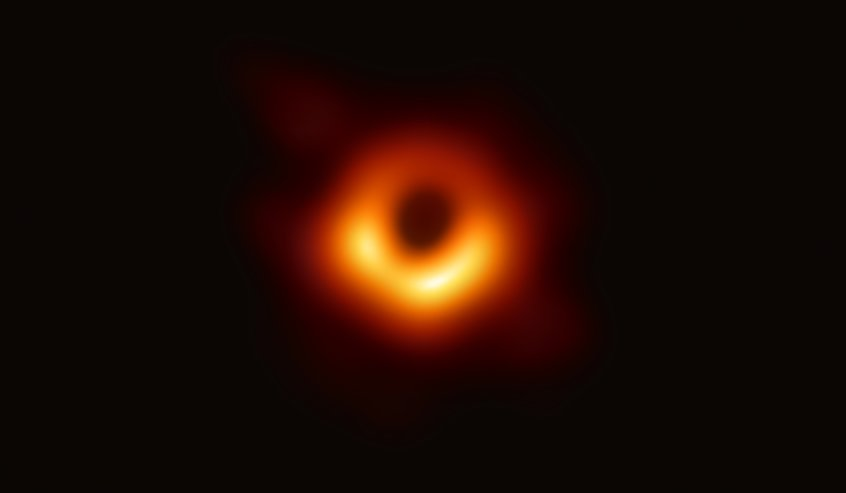
\includegraphics[width=10cm]{45456original.jpg}
    \caption{IMAGE OF BLACK HOLE M87}
    \label{fig:FIGURE 1}
\end{figure}
Earlier people used to think black holes are not real and considered it as an PSEUDOSCIENCE but with the help of AI we were able to compress ultra large image of black hole which provided the proof for the existence of  BLACK HOLES
\href{ https://numpy.org/case-studies/blackhole-image/}{FOR MORE INFO CLICK HERE}
\begin{figure}[htp]
    \centering
    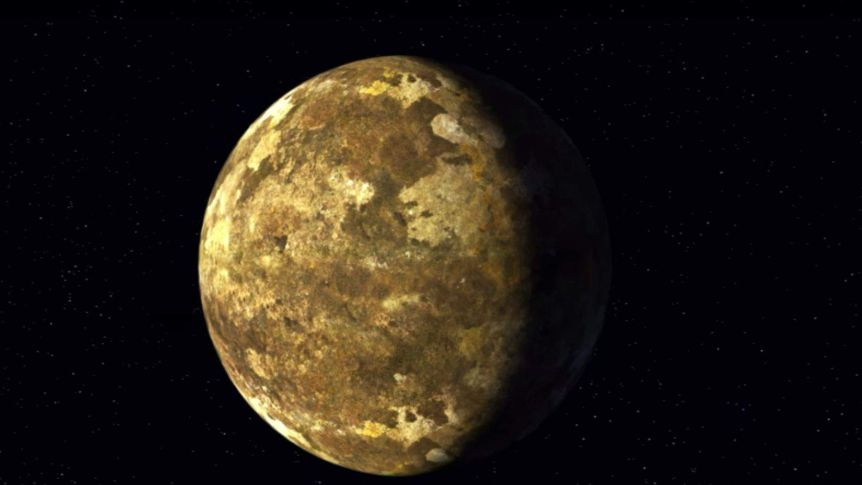
\includegraphics[width=10cm]{957149261348-16x9-xlarge.jpg}
    \caption{Kepler 90i}
    \label{fig:FIGURE 2}
\end{figure}
\\NASA’s Kepler Telescope was designed to determine the frequency of Earth-sized planets orbiting Sun-like stars, but these planets were on the very edge of the mission’s detection sensitivity. Accurately determining the occurrence rate of these planets required automatic and accurate assessing the likelihood that individual candidates are indeed planets, even at a low signal to noise ratio.

To overcome this limitation, researchers from Google and other scientists used a Convolutional Neural Network named AstroNet K2 to predict whether a given signal from Kepler’s space telescope is a transiting exoplanet or a false positive caused by the astrophysical or instrumental phenomenon. By training this neural network model up to 98(approx) percent, they successfully identified two new exoplanets namely Kepler 80g and Kepler 90i orbiting Kepler 80 star system and Kepler 90 star system respectively.
\href{https://www.nasa.gov/press-release/artificial-intelligence-nasa-data-used-to-discover-eighth-planet-circling-distant-star}{FOR MORE INFO CLICK HERE}
\end{document}
